\documentclass[aspectratio=169]{beamer}
\usepackage[T1]{fontenc}
\usepackage[utf8]{inputenc}
\usepackage[english,slovak]{babel}

\usepackage{amsmath}
\usepackage{amsthm}
\usetheme{Pittsburgh}
\useoutertheme{shadow}

\usepackage{graphicx}
\usepackage{caption}
\usepackage{subcaption}

\usepackage[]{algorithm2e}
\usepackage{listings}
 \setbeamercovered{transparent}
 \usepackage{cuted}
\usepackage[export]{adjustbox}
\usepackage{mathtools}

\usepackage{lipsum}
\usepackage{verbatim}
\usepackage{transparent}
\usepackage{framed}
\usepackage{xcolor}

\usepackage{multirow}
\usepackage{colortbl}
\usepackage{lmodern}

\usepackage{movie15}

\newcommand\Wider[2][3em]{%
\makebox[\linewidth][c]{%
  \begin{minipage}{\dimexpr\textwidth+#1\relax}
  \raggedright#2
  \end{minipage}%
  }%
}






\iftrue

\usetheme{Warsaw}

\setbeamercolor{normal text}{fg=white,bg=black!90}
\setbeamercolor{structure}{fg=white}

\setbeamercolor{alerted text}{fg=red!85!black}

\setbeamercolor{item projected}{use=item,fg=black,bg=item.fg!35}

\setbeamercolor*{palette primary}{use=structure,fg=structure.fg}
\setbeamercolor*{palette secondary}{use=structure,fg=structure.fg!95!black}
\setbeamercolor*{palette tertiary}{use=structure,fg=structure.fg!90!black}
\setbeamercolor*{palette quaternary}{use=structure,fg=structure.fg!95!black,bg=black!80}

\setbeamercolor*{framesubtitle}{fg=white}

\setbeamercolor*{block title}{parent=structure,bg=black!60}
\setbeamercolor*{block body}{fg=black,bg=black!10}
\setbeamercolor*{block title alerted}{parent=alerted text,bg=black!15}
\setbeamercolor*{block title example}{parent=example text,bg=black!15}

\fi









%-------------------------------------------------------------------------------------


\setbeamertemplate{navigation symbols}{}
\setbeamertemplate{footline}{}

%\setbeamertemplate{footline}[frame number]{}

\setbeamersize{text margin left=2mm,text margin right=2mm} 


\date[EURP]{}
\begin{document}

{
    \usebackgroundtemplate
    {
        \vbox to \paperheight{\vfil\hbox to \paperwidth{\hfil

        {\includegraphics[width=5.05in]{../images/rl_square.jpg}}

        \hfil}\vfil}
    }
   
}




\begin{frame}{\bf \hfill fast line following}

\begin{columns}

    \begin{column}{0.55\textwidth}


    \end{column}

    \begin{column}{0.45\textwidth}


      \begin{itemize}
          \setlength\itemsep{5em}
          \item {\bf baseline}
            \begin{itemize}
              \item constant speed
              \item PD controller for steering
              \item PIDs for motors controll
            \end{itemize}

          \item {\bf neural network}
            \begin{itemize}
              \item automatic target speed estimating using convolutional neural network
              \item real time curve shape classification (200Hz)
              \item robot can accelerate on straight line
            \end{itemize}
      \end{itemize}

 
    \end{column}


\end{columns}

\end{frame}




\begin{frame}{\bf \hfill steering controll quality}

\begin{columns}

    \begin{column}{0.7\textwidth}


    \end{column}

    \begin{column}{0.3\textwidth}

      \begin{itemize}
          \setlength\itemsep{2em}
          \item PD controller for steering
          \item two PIDs for motors controll
      \end{itemize}

 
    \end{column}

\end{columns}

\end{frame}





\begin{frame}[t]{\bf \hfill other features}


\begin{columns}

    \begin{column}{0.7\textwidth}

    \end{column}

    \begin{column}{0.3\textwidth}

      \begin{itemize}
          \setlength\itemsep{1em}
          \item broken line search
          \item color line following
      \end{itemize}

       \vfill

    \end{column}


\end{columns}

\end{frame}




\begin{frame}{\bf hardware}

\begin{columns}

    \begin{column}{0.5\textwidth}

        \begin{figure}
            \includegraphics[scale=0.3]{../images/motoko_uprising_hw.png}
        \end{figure}

    \end{column}

    \begin{column}{0.5\textwidth}

       \begin{itemize}
          \item MCU stm32f303, ARM Cortex M4F
            \begin{itemize}
              \item 72MHz
              \item 32bit floating point unit
              \item SIMD DSP instructions for deep learning
            \end{itemize}
          \item POLOLU micro metal gear motors
            \begin{itemize}
              \item gear ratio 1:30
              \item 180 pulses quadrature encoders
              \item DRV8834 H-Bridge driver
            \end{itemize}
          \item Sensors
            \begin{itemize}
              \item 8x phototransistor + white LED, 540nm
              \item 3xIR leds for obstacle detection
              \item gyroscope + accelerometer, LSM6DS0
            \end{itemize}
      \end{itemize}

 
    \end{column}

\end{columns}

\end{frame}



\begin{frame}{\bf 3D model for simulations}

  \begin{figure}
    \includegraphics[scale=0.35]{../images/robot_model.png}
  \end{figure}

\end{frame}


\begin{frame}{\bf PCB - top layer}

  \begin{figure}
    \includegraphics[scale=0.7]{../images/top.png}
  \end{figure}

\end{frame}

\begin{frame}{\bf PCB - bottom layer}

  \begin{figure}
    \includegraphics[scale=0.7]{../images/bottom.png}
  \end{figure}

\end{frame}


\begin{frame}{\bf PCB - design}

  \begin{figure}
    \includegraphics[scale=0.7]{../images/board.png}
  \end{figure}

\end{frame}


\begin{frame}{\bf assembling process}

  \begin{figure}
    \includegraphics[scale=0.09]{../images/IMG_20190701_153521.jpg}
  \end{figure}

\end{frame}


\begin{frame}{\bf assembling process - soldering detail}

  \begin{figure}
    \includegraphics[scale=0.09]{../images/IMG_20190701_153600.jpg}
  \end{figure}

\end{frame}


\begin{frame}{\bf assembling process - motor connection}

  \begin{figure}
    \includegraphics[scale=0.09]{../images/IMG_20190701_155139.jpg}
  \end{figure}

\end{frame}


\begin{frame}{\bf assembling process - complete robot}

  \begin{figure}
    \includegraphics[scale=0.09]{../images/IMG_20190701_161143.jpg}
  \end{figure}

\end{frame}





\begin{frame}{\bf software}

\begin{itemize}
  \item robot firmware is very complex - {\color{red} \bf thousands of lines} of C++ code
  \item there is custom C++11 templates {\color{red} hardware abstraction layer}
  \item custom {\color{red} event driven operating system} - all sensors tasks are running on background
  \item programmed without IDE, just simple text editor, \\
    {\color{red} sources are availible on} : \\
    https://github.com/michalnand/motoko\_uprising
\end{itemize}

\end{frame}


\begin{frame}[b]{\bf controll process}

  \vfill
  
  \begin{figure}[b!]
    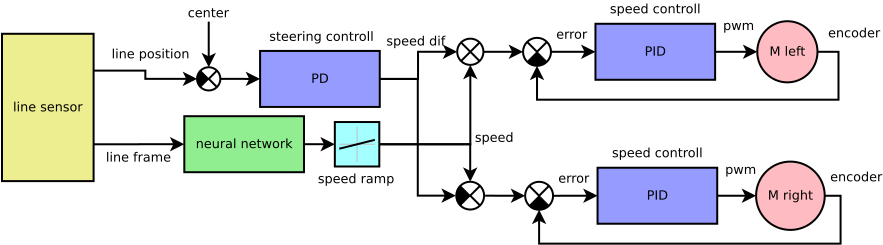
\includegraphics[scale=0.2]{../diagrams/lf/line_following.png}
  \end{figure}

\end{frame}



\begin{frame}[b]{\bf controll process - sensor reading}

\begin{enumerate}
  \setcounter{enumi}{0}
  \item the {\color{red} \bf line sensors} are readed using ADC \\
\end{enumerate}

  \vfill

  \begin{figure}[b!]
    \includegraphics[scale=0.2]{../diagrams/lf/line_following_01.png}
  \end{figure}

\end{frame}


\begin{frame}[b]{\bf controll process - sensor reading}

\begin{enumerate}
  \setcounter{enumi}{0}

  \item the {\color{red} \bf line sensors} are readed using ADC \\
    - thanks quadratic position interpolation, it provides 512 possible line positions
\end{enumerate}

  \vfill

  \begin{figure}[b!]
    \includegraphics[scale=0.2]{../diagrams/lf/line_following_01.png}
  \end{figure}

\end{frame}


\begin{frame}[b]{\bf controll process - neural network}

\begin{enumerate}
  \setcounter{enumi}{1} 
  \item the {\color{red} \bf neural network} performs curve shape classification
\end{enumerate}

 \vfill

  \begin{figure}
    \includegraphics[scale=0.2]{../diagrams/lf/line_following_02.png}
  \end{figure}

\end{frame}


\begin{frame}[b]{\bf controll process - neural network}

\begin{enumerate}
  \setcounter{enumi}{1}
  \item the {\color{red} \bf neural network} performs curve shape classification
    \begin{itemize}
      \item input is matrix, 8x8, eight past line sensors readings
      \item output is one of 5 classes : \\
        sharp left,  soft left, center line, soft right, or sharp right
      \item network runtime is only 2 miliseconds
    \end{itemize}
\end{enumerate}

 \vfill


 \begin{columns}

    \begin{column}{0.5\textwidth}

      \begin{figure}
        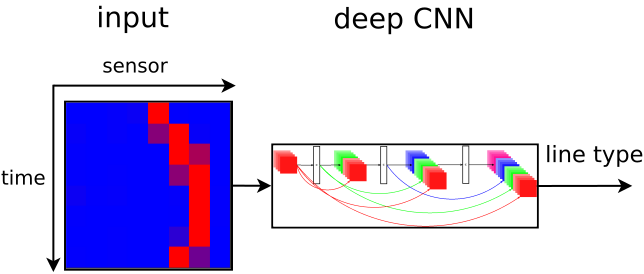
\includegraphics[scale=0.2]{../diagrams/line_classification.png}
      \end{figure}

    \end{column}

    \begin{column}{0.5\textwidth}

      \begin{figure}
        \includegraphics[scale=0.15]{../diagrams/lf/line_following_02.png}
      \end{figure}

    \end{column}

\end{columns}



\end{frame}



\begin{frame}[b]{\bf controll process - steering}

\begin{enumerate}
  \setcounter{enumi}{2}
  \item the {\color{red} \bf steering} PD controller compute speed difference
\end{enumerate}

 \vfill

  \begin{figure}
    \includegraphics[scale=0.2]{../diagrams/lf/line_following_03.png}
  \end{figure}

\end{frame}


\begin{frame}[b]{\bf controll process - steering}

\begin{enumerate}
  \setcounter{enumi}{2}
  \item the {\color{red} \bf steering} PD controller compute speed difference \\
    - of course, the filtered derivative term is used
\end{enumerate}

 \vfill

  \begin{figure}
    \includegraphics[scale=0.2]{../diagrams/lf/line_following_03.png}
  \end{figure}

\end{frame}



\begin{frame}[b]{\bf controll process - motors controll}

\begin{enumerate}
  \setcounter{enumi}{2}
  \item the {\color{red} \bf motors speed} is controlled with two PIDs
\end{enumerate}

 \vfill

  \begin{figure}
    \includegraphics[scale=0.2]{../diagrams/lf/line_following_04.png}
  \end{figure}

\end{frame}


\begin{frame}[b]{\bf controll process - motors controll}

\begin{enumerate}
  \setcounter{enumi}{2}
  \item the {\color{red} \bf motors speed} is controlled with two PIDs \\
    - PIDs are using antiwindup, so the response looks quick
\end{enumerate}

 \vfill


\begin{columns}

    \begin{column}{0.5\textwidth}

      \begin{figure}
        \includegraphics[scale=0.2]{../images/motor_controll.png}
      \end{figure}

    \end{column}

    \begin{column}{0.5\textwidth}

  \begin{figure}
    \includegraphics[scale=0.15]{../diagrams/lf/line_following_04.png}
  \end{figure}

    \end{column}

\end{columns}


\end{frame}





\begin{frame}[t]{\bf \hfill end to end line follower}

\begin{columns}

    \begin{column}{0.55\textwidth}

    \end{column}

    \begin{column}{0.45\textwidth}

      \begin{itemize}
          \setlength\itemsep{0.5em}
          \item {\bf \color{red} reinforcement learning} line follower
      \end{itemize}

       \vfill

    \end{column}


\end{columns}

\end{frame}



\begin{frame}[t]{\bf \hfill end to end line follower}

\begin{columns}

    \begin{column}{0.55\textwidth}

    \end{column}

    \begin{column}{0.45\textwidth}

      \begin{itemize}
          \setlength\itemsep{0.5em}
          \item {\bf \color{red} reinforcement learning} line follower
          \item {\bf \color{red} no PD, PIDs, no dataset} \\ 
          -just learned from rewards and pushments
      \end{itemize}

       \vfill

    \end{column}


\end{columns}

\end{frame}




\begin{frame}[t]{\bf \hfill end to end line follower}

\begin{columns}

    \begin{column}{0.55\textwidth}

    \end{column}

    \begin{column}{0.45\textwidth}

      \begin{itemize}
          \setlength\itemsep{0.5em}
          \item {\bf \color{red} reinforcement learning} line follower
          \item {\bf \color{red} no PD, PIDs, no dataset} \\ 
          -just learned from rewards and pushments
          \item {\bf \color{red} self understand} what the line is, what the goal is ...
      \end{itemize}

       \vfill

    \end{column}


\end{columns}

\end{frame}





\begin{frame}[t]{\bf \hfill end to end line follower}

\begin{columns}

    \begin{column}{0.55\textwidth}

    \end{column}

    \begin{column}{0.45\textwidth}

      \begin{itemize}
          \setlength\itemsep{0.5em}
          \item {\bf \color{red} reinforcement learning} line follower
          \item {\bf \color{red} no PD, PIDs, no dataset} \\ 
          -just learned from rewards and pushments
          \item {\bf \color{red} self understand} what the line is, what the goal is ...
          \item {\bf \color{red} advantage actor critic} algorithm
      \end{itemize}

       \vfill

    \end{column}


\end{columns}

\end{frame}




\begin{frame}[t]{\bf \hfill end to end line follower}

\begin{columns}

    \begin{column}{0.55\textwidth}

    \end{column}

    \begin{column}{0.45\textwidth}

      \begin{itemize}
          \setlength\itemsep{0.5em}
          \item {\bf \color{red} reinforcement learning} line follower
          \item {\bf \color{red} no PD, PIDs, no dataset} \\ 
          -just learned from rewards and pushments
          \item {\bf \color{red} self understand} what the line is, what the goal is ...
          \item {\bf \color{red} advantage actor critic} algorithm
          \item here is the magic 
            \begin{align*} 
              \mathcal{L} = &(V - \hat{V})^2 + \\
                     &-log(p(A|S))(V - \hat{V}) \\
                     &-\beta \mathcal{H}(A)
            \end{align*}
      \end{itemize}

       \vfill

    \end{column}


\end{columns}

\end{frame}



\begin{frame}{}

\centering
{\bf Thanks for watching}

\end{frame}



\end{document}
